\documentclass{article}
\usepackage[utf8]{inputenc}
\usepackage[T1]{fontenc} 
\usepackage[english]{babel}

\usepackage{amsmath,amsthm}
\usepackage{amsmath,amssymb}
\usepackage{amsfonts}
\usepackage{mathtools}
\usepackage{newtxtext}
\usepackage{newtxmath}

\usepackage{geometry}

\usepackage{microtype}
\usepackage{floatflt}

\usepackage{graphicx}

\usepackage{hyperref}
\usepackage[backend=bibtex]{biblatex} %I need to use biblatex for some special features

\date{\today}
\author{Neil \& Enrique, Erik Pillon}
\title{Finite Elements Project}

\usepackage{mdframed}
\mdfsetup{skipabove=\topskip,skipbelow=\topskip}
\global\mdfdefinestyle{exampledefault}{%
outerlinewidth=5pt,innerlinewidth=0pt,outerlinecolor=red,roundcorner=5pt
}

% AMBIENTI MATEMATICI
\newcommand{\R}{\mathbb{R}}
\newcommand{\C}{\mathbb{C}}
\newcommand{\tu}{\tilde{U}}
\renewcommand{\hat}{\widehat}
\renewcommand{\phi}{\varphi}
\newcommand{\diff}{\mathop{}\!d}
\newcommand{\norm}[1]{\left\lvert #1\right\rvert}
\newcommand{\pd}[2]{\frac{\partial #1}{\partial #2}}
\newcommand{\pds}[2]{\frac{\partial^2 #1}{\partial #2^2}}

% IMPORTARE CODICE IN MATLAB/OCTAVE
\usepackage{listings}
\usepackage{color}

\begin{document}
\maketitle
\begin{abstract}
	This is the final project of the course \textbf{Numerical Methods}, given at Phelma in the Academic Year 2017/2018. In this project we will study a process of material elaboration involving heating by electrode. We 'll study the steady state of this process. The objective is to model the physical phenomena which take place in this process with \emph{finite element method}.
\end{abstract}
\section{Statement of the Problem}
The study configuration is considered cylindrical. A scheme of the study geometry is given in Figure~\ref{figure:problem}:
\begin{figure}
	\centering
	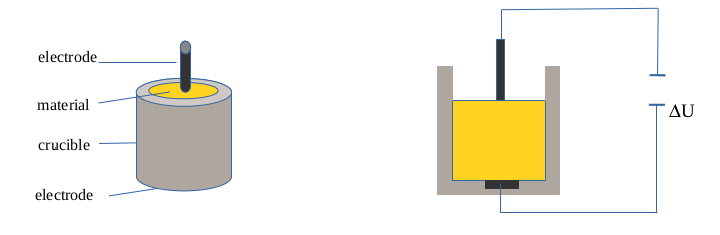
\includegraphics[height=4cm]{Images/problem.png}
	\caption{Problem Scheme}
	\label{figure:problem}
\end{figure}
The process is constituted by:
\begin{itemize}
	\item a cylindrical crucible;
	\item the elaborated material; the geometry of the study domain occupied by the material is cylindrical;
	\item 2 electrodes.
\end{itemize}

The electrodes are in graphite. An electrical potential difference is applied between the top electrode and the bottom electrode included in the crucible: $ \Delta U $. This electrical potential difference is \emph{continuous}. An electrical current pass through the material placed in the crucible. We suppose that the contact between the electrodes and elaborated material is perfect. \textbf{Joule effect heat the material}. The material of the crucible is an insulating material. The crucible is not model and will be replaced by an adapted boundary condition. Electrical problem has to be solved in the electrodes and in the elaborated material. The heat transfer has to be solved in the material only.

\section{Equations of the physical phenomenon and Boundary Conditions}
The objective of this part is to present the physical equations of the process in the steady state and boundary conditions. In this process two physical phenomena occur:
\begin{itemize}
	\item electrical phenomenon;
	\item thermal phenomenon.
\end{itemize}
\subsection{Presentation of the study domain}
Describe the study domain. Precise where each phenomenon is solved.
\begin{mdframed}
	The study domain is the one described in Figure~\ref{figure:problem}, right part. 
	\begin{itemize}
		\item We will solve the \textbf{thermal problem} only in the material only (yellow part), i.e.~where $ 0.1<r<0.3 $ and $ 0<h<0.3 $.
		\item We will solve the \textbf{electrical problem} in the electrodes and in the elaborated material, i.e.~for $ 0\geq r<0.3 $ and $ 0<h<0.3 $.  
	\end{itemize} 
\end{mdframed}
\subsection{Electrical problem}
Give the partial differential equation of the electrical problem.
Give the boundary conditions of the electrical problem.
Give the expression of the current density and of the Joule power density.
\begin{mdframed}
	
\end{mdframed}

\subsection{Thermal problem}
\begin{itemize}
	\item Give the partial differential equation of the thermal problem.
	\item Give the boundary conditions of the thermal problem.
\end{itemize}
\begin{mdframed}
	The Fourier Law tells us that:
	\begin{equation}
	\label{eq:Fourier}
	q=-k\nabla T
	\end{equation}
	where
	\begin{description}
		\item[$ q$] local heat flux density,
		\item[$ k $] material's conductivity,
		\item[$ \nabla T $] is the temperature gradient. 
	\end{description}
	From the Gauss-Green theorem we know that 
	\[
	\iint_S q(x,y,z) \diff S=Q
	\]
	where the first integral is all over the surface defined by $ 0.1<r<0.3 $ and $ 0<h<0.3 $ and $ Q $ is the heat generated by the Joule effect.
	
	By the way, employing the divergence theorem, the left hand side of the equation can be rewritten as  
	\[ \iiint \nabla\cdot q(x,y,z) \diff x\diff y\diff z = \iint_S q(x,y,z) \diff S  \]
	and then the following identity holds
	\begin{equation}
	\iiint \nabla\cdot q(x,y,z) \diff x\diff y\diff z = Q.
	\end{equation}
	Using Fourier Law \eqref{eq:Fourier} and plugging it into the above equation we obtain
	\begin{equation}
	\nabla\cdot(-k\nabla T)=Q.
	\end{equation}
\end{mdframed}

	
\section{Principle of the Modeling}
\begin{mdframed}
	In this project, in a first step, each equation will be developed and test. In a second step, the model with the
	two coupling equations will be developed and test. For numerical modeling the finite element method is
	used. In this project, describe the steps of the calculation and the variables used. Take time to define how you
	will present your numerical results.
\end{mdframed}



\end{document}
